
\chapter{Programming Model}\label{ch:prog}

\section{Object Layout}

\unedit{
    Objects in Twizzler often have a header at the object's base, the contents of which depend on what
    the object contains. Often these headers have pointers to other data in the object, and describe the
    type of the object. For example, in our evaluation we implement a red-black tree in an object. The
    header contains some basic information about the tree as well as a pointer to the root node. Placing
    headers at the object's base gives applications a ``starting point'' that they can use to start
    accessing object data. Twizzler provides a dedicated function to get a pointer to an object's
    header, called \texttt{obj\_base}.

    Note that the base address of an object is \emph{not} at offset 0, but instead one page up, so that we
    can still trap NULL pointers. If this were not the case, a pointer value of 0 would still be a valid
    pointer, and we want to remain backwards compatible with the assumption that a NULL pointer has
    integer value 0. The bottom page of an object is unmapped by Twizzler, allowing NULL pointer
    dereferences to be trapped by the kernel.

    While objects are flat, contiguous regions of memory, different applications may want to organize
    that memory in different ways. Some objects, such as \texttt{views} are largely interpreted as an
    array, but sometimes applications need to explicitly allocate and deallocate memory within an object.
    Twizzler provides an API to allocate and free units of memory from application-specified regions
    within objects. We make use of this in our red-black tree code, where new nodes are allocated out of
    the object using this API.

    Figure~\ref{fig:typobj} shows a typical object in Twizzler. The NULL page is always present to trap
    NULL pointers, and is followed by a header. The application setting up this object may have a region
    of some contiguous data (such as some strings, or an array), and may point to it from the header.
    The object may have a region setup for allocation so that a future application using this
    object can easily allocate and free memory when manipulating the object. Finally, the FOT and
    metadata regions start at the top of the object and grow downwards.
    \begin{SCfigure}
        \centering
        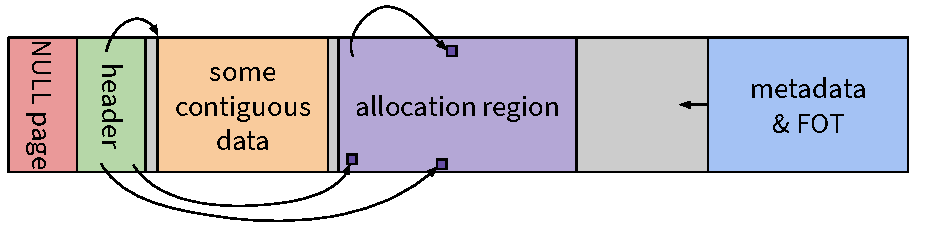
\includegraphics[width=\linewidth]{fig/typobj}
        \caption{A typical object layout. The header, contiguous region, and allocation region are all
            optional, however most objects will have a header. This object contains a number of internal
            pointers between regions. The metadata region (which includes the FOT) grows downward.}
        \label{fig:typobj}
    \end{SCfigure}
}

\section{Memory Safety and Lifetimes}


\unedit{

    \paragraph{Object Types, Persistence, and Lifetime}

    Applications need to be able to specify what \emph{type} of memory an object resides in. Currently,
    we are operating on systems that contain both persistent \NVM and volatile DRAM as main memory, and
    applications may want to make use of both of these memory types. Placing certain objects in DRAM,
    for example, can result in performance improvements (\eg caching read-only objects) or security
    improvements (\eg making temporary key material volatile). \Twizzler exposes this choice to
    applications at object creation time, allowing them to specify the type of the object. At least two
    types, \emph{volatile} and \emph{persistent}, are supported by default. As additional types of physical memory
    are added to systems (\eg different kinds of \NVM with different properties, high-bandwidth memory,
    \etc), applications may wish to have more fine-grained control over where objects are placed, and
    \Twizzler's APIs allow such control. Objects can also be moved between types of memory after
    creation, though this may be a time consuming operation as it involves copying potentially large
    amounts of data.

    By default, objects are persistent and live in kernel-managed \NVM unless they are marked as
    volatile. If an object is volatile, it has a limited lifetime that is related to the power state of
    the machine---as soon as power is lost (or the system is rebooted) all volatile objects disappear.
    Note that \Twizzler removes the distinction between volatile and persistent objects for how
    applications \emph{access} data, relying on higher-level language or library support and application
    support for dealing with the limited lifetime of volatile objects.

    The property of persistent versus volatile for objects differs from the concept of
    ephemeral data. The ``volatile'' property places a physical restriction on the lifetime of an object (the machine's
    power state), while the ``persistent'' property indicates that the object will exist until
    explicitly deleted. Objects can also be long-lived or ephemeral independent of their persistence
    property, since we use the term ``ephemeral'' to describe information, data, or state that has a
    finite lifetime and is expected to ``go away''. While all volatile objects are ephemeral, the
    reverse is not true---we may place ephemeral data in a persistent object to allowed for recovery
    after an unexpected power cycle. The ``persistent'' property of an object is a recorded piece
    of information that the kernel associates with an object, but there is no such information for ephemeral
    versus long-lived. Instead, we provide a mechanism for specifying a logical lifetime of objects
    relative to one another with a mechanism called \emph{ties}, which we will discuss below.

    \paragraph{Object Ties and Logical Lifetime}

    \iffalse
        Objects are, by default, persistent and live in kernel-managed \NVM. During creation, an object may
        be marked as ``volatile'', allowing the kernel to allocate memory for it from DRAM. This is useful
        for temporary application data that does not need to be persistent, such as stacks or volatile
        heaps. At any time, an object may be changed from volatile to persistent, or vice versa, but this
        may be a time consuming operation. Note that, although \Twizzler does distinguish between volatile
        and persistent objects (and allows applications to choose based on some policy what their objects
        are), \Twizzler removes the distinction between them when it comes to accessing the data.

        Throughout the paper, we use both terms ``volatile'' and ``ephemeral'' for different purposes.
        Volatile is a property of hardware---the data goes away when power is lost. We expose this meaning
        in objects that are marked as ``volatile'' to allow application to capitalize on the benefits of
        volatile memory (both performance and security). Ephemeral, more broadly, describes information,
        data, or state that has a finite lifetime and may ``go away''. This is in contrast to persistent
        data which has an ``infinite'' lifetime, and volatile data which has a finite lifetime tied to the
        power state of the machine. All volatile objects are ephemeral, while the reverse is not necessarily
        true (\eg an application may have some temporary state that it makes persistent to recover from a
        power cycle).
    \fi

    %An example of ephemeral data is temporary application data like a stack or a heap.
    Applications in \Twizzler also have some lifetime; an application's job is typically to operate on
    some persistent data while performing some computation before eventually exiting. Such an
    application will likely use volatile objects to represent temporary computation state (\eg the
    stack and heap, which are ephemeral). However, just assigning an object as volatile is insufficient
    because there is a lifetime mismatch: the volatile object will live until the next reboot while the
    application may exit before then or may even live and try to recover after a power cycle. Simply
    manually deleting the volatile object when the application is done is also insufficient, as it does
    not account for crashes where the application may be unable to clean up its state. Furthermore,
    applications that wish to support recovery may make use of persistent stacks and heaps, thus these
    objects would have to be persistent despite being ephemeral.

    While we could provide a mechanism designed specifically for this ``system-level'' task,
    where the kernel maintains a set of objects to automatically cleanup when an application exits, this
    would require the kernel to have some understanding of what an ``application'' is. Furthermore, if
    we generalize a solution to automatic cleanup, we can allow applications to make use of it for their
    own purposes. For example, in \unix, it is common for programs to create and immediately unlink
    files to ensure the system frees those resources when the program exits. We would like to reproduce
    similar semantics here that also solves the lower level problem above of freeing application state
    by assigning a lifetime to objects that is more expressive than simply ``volatile'' and
    ``persistent''.

    \iffalse
        Applications need a mechanism to express the relative lifetime of objects in the system to ensure
        that a given object exists at least as long as another object. Specifying object lifetimes is
        commonly used to enable automatic cleanup. For example, in \unix, programs often create and
        immediately unlink files to ensure the system deletes them on exit. Similarly, a lot of ephemeral
        resources that applications typically use (\eg the stack, the heap) are formalized as objects in
        \Twizzler\footnote{Formalizing these resources as objects both simplifies the programming
            environment model and allows them to be optionally persisted, allowing applications to resume their
            state after crashes.}.
    \fi

    In \Twizzler, object lifetime is expressed through \emph{ties}.
    An object can be tied to another by invoking a system call that tells the kernel that
    object \texttt{A} is tied to object \texttt{B}, after which the lifetime of \texttt{A} is
    guaranteed to be at least that of \texttt{B}. The kernel will not fully delete object \texttt{A} (even if the
    delete system call is invoked on it) until after \texttt{B} is fully deleted. An object may be tied
    to a large (but finite) number of other objects and may also be \emph{untied} at any time. This
    model of specifying object lifetime relative to others is similar to Rust~\cite{rust}, where
    reference lifetime can be named so that the programmer can express lifetimes of objects relative to
    each other. Note that object ties are not related to persistent pointers (discussed in more detail
    in \S~\ref{sec:invariant_pointers}), and instead primarily provide a way to formalize automatic cleanup.


    Object ties provide a convenient mechanism for applications to build large data structures across
    multiple objects without giving up easy cleanup if something goes wrong or if the ``root'' object is
    deleted. \Twizzler also uses ties internally: when an object is created as copy-from an existing
    object, it uses copy-on-write semantics, and thus internally marks the source object as tied to the
    new object. We also tie ephemeral program state objects to threads (which are also represented by
    objects) such that they are automatically cleaned up when a program exits. It is our expectation
    that application programmers will only rarely directly use ties. Instead, we expect that ties will
    provide necessary features that higher-level programming language support for persistent memory can
    use.

    Note that object ties interact with the notion of volatile and persistent objects, because
    volatile objects have an implicit \emph{maximum} lifetime---that of the next machine restart or
    power loss. Tying volatile objects to volatile objects and persistent objects to persistent objects both act as
    expected. Tying a persistent object to a volatile object is also semantically simple (persistent
    objects already have an ``assumed lifetime'' that is longer than a volatile object). Tying a
    volatile object to a persistent object, however, may seem somewhat nonsensical. However, \Twizzler
    does still allow this because it has useful semantics: if an application creates a data structure
    with some volatile component\footnote{Since \Twizzler's kernel is not involved in reference
        creation, it cannot prevent such a reference from being created. We expect language support for
        persistent data structures to impose restrictions on applications in this regard, and the OS should
        not prematurely restrict how applications use volatile and persistent objects. Access to a volatile
        object that no longer exists after a reboot results in a simple access fault, mitigating security
        concerns.},
    %\footnote{We will discuss the implications of creating references
    %between volatile and persistent objects in \S~\ref{twz:pptr}.}
    it may want to tie the lifetime of that volatile component to the
    persistent component if the data structure is to be deleted. This use case (creating a persistent
    object that we expect to delete) is not uncommon, particularly in applications designed to recover
    partial computation after a crash. Note that, in this case, the maximum
    lifetime of the volatile object is still in-play; after a power cycle, that object will no longer be
    present, so tying a volatile object to a persistent object is somewhat dangerous.

}


\subsection{Safe Allocation}

\section{Transactions}


\unedit{

    \subsection{Crash Consistency}
    \label{sec:crash}
    \Twizzler provides primitives for building crash-consistent data structures. At a low level,
    it provides mechanisms for writing back cache-lines, appropriate fences, and basic transactions.
    Applications use these primitives today outside of \Twizzler to build up larger, more complex support for
    crash-consistent data structures.
    %, thus we provide similar primitives.


    Our goal is to provide low level primitives without restricting programs or prematurely
    prescribing particular solutions. There is a wealth of research on crash-consistent
    data structures for
    \NVM~\cite{condit:sosp09,coburn:asplos11,volos:asplos11,dulloor:eurosys14,narayanan:asplos12,ni:hotstorage18,ni:micro19,ogleari:hpca18,lu2014loose},
    but it is still in flux. Of course, \Twizzler manages \emph{system} data structures,
    such as FOT entries, views, \emph{etc.}, in a
    crash-consistent manner using the aforementioned primitives, locking, and fencing.


    \Twizzler also provides a transactional-persistent logging mechanism.
    Programmers can write \texttt{TXSTART}--\texttt{TXEND} blocks to denote transactions and \texttt{TXRECORD}
    statements to record pre-changed values. This is similar to the mechanism provided by
    PMDK~\cite{libpmem}. If applications need more complex
    transactions using different logging mechanisms, they can use libraries. \Twizzler's internal data
    structures and \libcore's manipulation of object metadata is handled via a combination of these
    transactions and cache-line writebacks.

    \Twizzler provides a mechanism for restarting threads when power is restored following a crash.
    Since views are persistent objects, all objects mapped during a thread's execution are known across
    power cycles, and are mapped back in. The thread is then started at a special \texttt{\_resume}
    entry point, allowing the program to handle the power failure in an application-specific manner.  Of
    course, \emph{volatile} objects will be lost when power resumes, and thus any attempted access to
    these objects will result in an exception. Thus applications that wish to resume after power failure
    will need to be aware of and handle this. We do not wish to prescribe any restrictions
    here---applications that want to place their heap in volatile memory for performance or security
    reasons should be allowed to. We expect higher level support for applications to manage persistent
    data, such as language support for persistent heaps, to make use of the features we provide, so
    applications that want to resume can put resuming information in persistent objects.

    The reason we choose to restart threads at a known, different entry point from normal application
    start up is that in current systems, there is always volatile computation state (\eg registers, the
    cache) that is lost when power is lost. Of course, in the future, systems may be able to prevent the
    loss of more and more ephemeral computation state (with the logical extreme being perfect
    resumability). In this case, the \texttt{\_resume} handler can be a simple stub that resumes the
    execution exactly as left off. The more likely case, periodic checkpointing, can be similarly
    handled, with the \texttt{\_resume} handler selecting the most recent valid check point to resume
    from. The \texttt{\_resume} handler enables all of these solutions, thus remaining applicable across
    hardware evolution.

}